% Shared preamble for the English summaries in this repository.
\documentclass[11pt,a4paper]{article}
\usepackage[margin=2.2cm]{geometry}
\usepackage[T1]{fontenc}
\usepackage[utf8]{inputenc}
\usepackage{lmodern}
\usepackage{amsmath,amssymb}
\usepackage{graphicx}
\usepackage{booktabs}
\usepackage{enumitem}
\usepackage[hidelinks]{hyperref}
\setlist{itemsep=2pt,topsep=4pt}
\setlength{\parindent}{0pt}
\setlength{\parskip}{5pt}
\graphicspath{{figures/}}
\newcommand{\summaryheader}[3]{%
  \begin{center}
    {\Large\bfseries #2}\\[3pt]
    {\large #1}\\[3pt]
    {\small Arshia Goshtasbi \textbullet{} MSc Electrical Engineering (Control), Iran University of Science and Technology \textbullet{} #3}
  \end{center}
  \vspace{2pt}\hrule\vspace{8pt}
  \noindent\textit{English summary of my original Persian report, which is kept as a PDF in this folder.}\par}

\begin{document}
\summaryheader{Adaptive Control, Homework 5}{Model-reference Adaptive Systems (Åström \& Wittenmark, Examples 5.1, 5.2 and 5.7)}{Autumn 1404 (2025)}

All cases are subsystems of \texttt{HW5.slx}. Each was simulated for three adaptation gains $\gamma$ and compared with the book.

\begin{description}
  \item[Example 5.1: MIT rule, adapting a feed-forward gain.] $\gamma=0.5$, $1$, $2$. In the re-run, the gain estimate settles in every case; with larger $\gamma$ it moves faster and oscillates more before settling.
  \item[Example 5.2: MIT rule for a first-order plant with two parameters.] $\gamma=0.2$, $1$, $5$. I plotted the output, the control signal and the estimates $\theta_1$, $\theta_2$.
  \item[Example 5.7: Lyapunov-based MRAS for the same plant.] $\gamma=0.2$, $1$, $5$. The update law is derived from a Lyapunov function instead of the MIT gradient rule.
\end{description}

\begin{center}
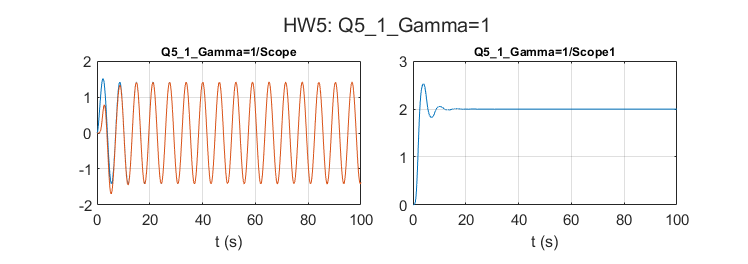
\includegraphics[width=0.48\linewidth]{Q5_1_gamma1.png}\hfill
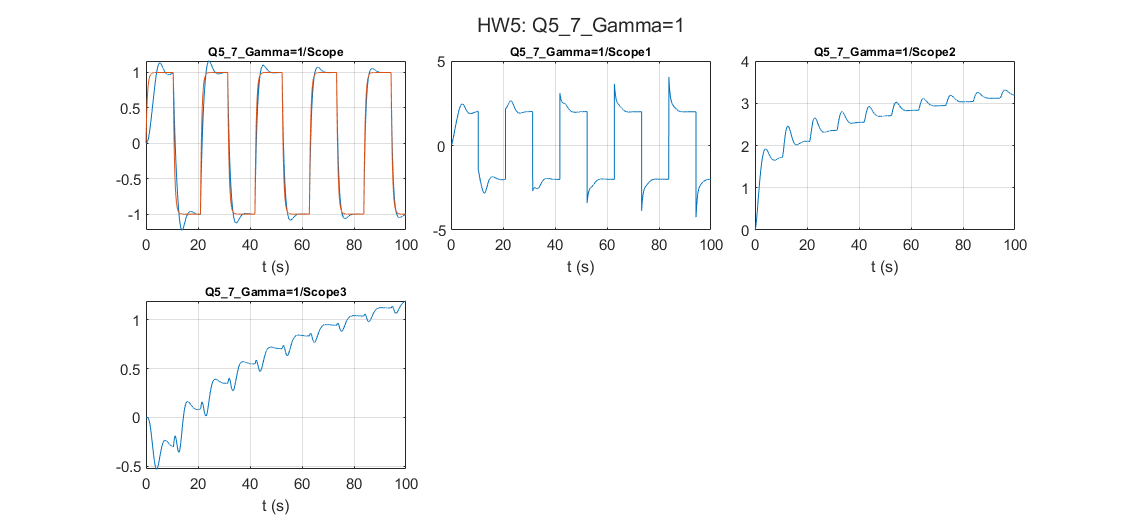
\includegraphics[width=0.48\linewidth]{Q5_7_gamma1.png}\\[2pt]
{\small Re-run in R2023b: example 5.1 (left) and example 5.7 (right), both with $\gamma=1$.}
\end{center}
\end{document}
